% Options here are passed to the article class.
% Most common options: 10pt, 11pt, 12pt
\documentclass[10pt]{datasheet}

% Input encoding and typographical rules for English language
\usepackage[utf8]{inputenc}
\usepackage[english]{babel}
\usepackage[english]{isodate}

% tikz is used to draw images in this example, but you can
% also use \includegraphics{}.
\usepackage{graphicx}
\usepackage{float}
\usepackage{subcaption}

% These define global texts that are used in headers and titles.
\title{SG04: Compact Shulker Box Splitter Array}
\author{Basil, Kizu}
\tags{splitting}
\date{25 December 2024}
\revision{Revision 1}
\begin{document}
\maketitle

\section{Features}
% FHL
% Unstackable Separation
% 100% empty box collection reliability (Breaks into the top most water stream which makes it not need an isbox at the unstackable output)
% Fast assignment of boxes
% Empty box call already setup
% Incredibly small
% Filter itemless (kissing hoppers)
% Pausable (Will break sorted boxes if running) Assignment/Filter Clock
% If it runs out of empty boxes the hoppers will unlock automatically for a refill
\begin{itemize}
\item{Compact design. 20x17x7}
\item{Seperate output for unstackable items.}
\item{Fully hopperlocked.}
\item{Filter itemless. (kissing hoppers)}
\item{Pausable. Will only break sorted boxes if running.}
\item{Automatic refill of empty boxes.}
\item{Will ensure empty boxes are present before starting and will pause if empty boxes run out.}
\end{itemize}

\section{Applications}

\begin{itemize}
\item{Splitting mixed item shulker boxes for dynamic sorting systems.}
\end{itemize}

\section{General Description}
The SG04 is a compact shulker box splitter array that can split mixed item shulker boxes into smaller boxes of the same type. The design uses the hopper dueling mechanism for a "filter itemless" setup. It uses a global clock to allow for it to be paused during operation. Note: It is not empty box input proof. Inspired by Obi's design.
\vfill\break

\begin{figure}[H]
    \centering
    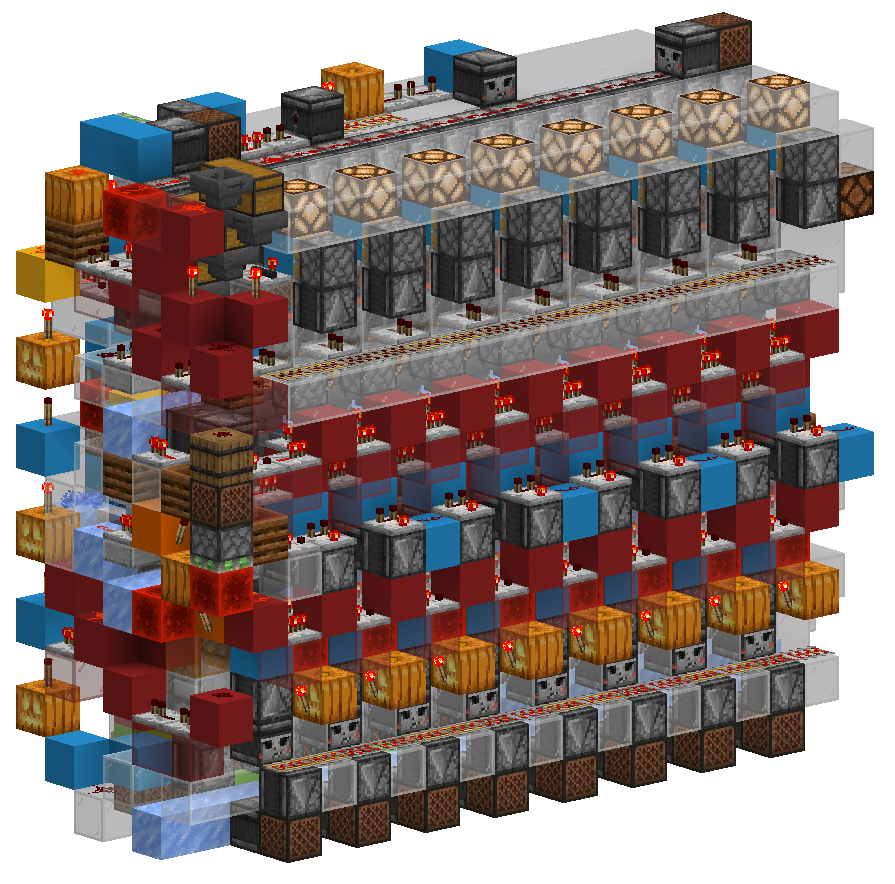
\includegraphics[width=0.48\textwidth]{area_render_20_.png}
    \caption{\centering Compact Shulker Box Splitter Array}
\end{figure}

% For wide tables, a single column layout is better. It can be switched
% page-by-page.
\onecolumn

\section{Device Specifications}

\begin{table}[H]
    \caption{Inputs}
    \begin{tabularx}{\textwidth}{l | c | X}
        \thickhline
        \textbf{Name} & \textbf{Range} & \textbf{Description} \\
        \hline
        Mixed boxes input & Box & Boxes to split. Boxes can contain any items. \\
        \hline
        Empty boxes input & Box & Empty boxes for loading. (waterstream) \\
        \hline
        Start processing & Pulse & Starts processing mixed boxes. \\
        \hline
        Pause & 0-1 & Pauses the device. \\
        \thickhline
\end{tabularx}
\end{table}

\begin{table}[H]
    \caption{Outputs}
    \begin{tabularx}{\textwidth}{l | c | X}
        \thickhline
        \textbf{Name} & \textbf{Range} & \textbf{Description} \\
        \hline
        Split boxes output & Box & Boxes with same item types only \\
        \hline
        Unstackables output & Item & Unstackable items \\
        \hline
        Empty boxes output & Box & Empty boxes from unloading \\
        \thickhline
\end{tabularx}
\end{table}

\begin{table}[H]
    \caption{Device Specifications}
    \begin{tabularx}{\textwidth}{l | c c c | c | X}
        \thickhline
        \textbf{Parameter} & \textbf{Min.} & \textbf{Typ.} & \textbf{Max.} &
        \textbf{Unit} & \textbf{Conditions} \\
        \hline
        MC Version & 1.16 & 1.21.4 & - & MCV & Latest version at time of writing: 1.21.4\\
        \hline
        Dimensions & & 20 x 17 x 7 & & Blocks & \\
        \thickhline
\end{tabularx}
\end{table}

\section{Testing Data}
\begin{table}[H]
    \caption{Executed Tests}
    \begin{tabularx}{\textwidth}{l | X}
        \thickhline
        \textbf{Test} & \textbf{Result} \\
        \hline
        Splitting test & Device was able to split mixed boxes correctly. \\
        \thickhline
\end{tabularx}
\end{table}
\section{Download Information}
\begin{table}[H]
    \caption{Download Information}
    \begin{tabularx}{\textwidth}{l | l | l | X}
        \thickhline
        \textbf{Identifier} & \textbf{MC} & \textbf{File} & \textbf{Description} \\
        \hline
        SG04 & 1.21.4 & \href{https://github.com/Soontech-Annals/Archive/blob/2b73adfd252c5e2cf9d202454dbef78a586bc482/Archive/splitting/SG04\%20Compact\%20Shulker\%20Box\%20Splitter\%20Array/SG04\_Compact\_Shulker\_Box\_Splitter\_Array.litematic?raw=1}{SG04\_Compact\_Shulker\_Box\_Splitter\_Array.litematic} & Schematic of device. \\
        \hline
        \thickhline
    \end{tabularx}
\end{table}


\section{Related Components}
\begin{table}[H]
    \caption{Related Components}
    \begin{tabularx}{\textwidth}{ l | l }
        \thickhline
        \textbf{Identifier} & \textbf{Description} \\
        \hline
        SG02 & Global Clock Shulker Box Splitter \\
        \thickhline
    \end{tabularx}
\end{table}

\end{document}

